\chapter{Introduction to PDEs and Numerical Methods for Solving Them}

In the rest of the course we turn our attention to the numerical 
solution of PDEs, i.e., differential equations that 
involve partial derivatives of a function. In the case of 
ODEs we always dealt with problems of the form 
\begin{equation*}
    u'(t) = f(t,u), \quad \text{plus boundary cond.}
\end{equation*}
where $u: [a,b] \to \R \; {\rm or} \; \C$, i.e., $u$ only depends on 
a scalar input which we think of as time or space. For PDEs, 
$u$ will typically depend on multiple variables and so partial 
derivatives with respect to each input coordinate have to be 
considered. 

We will consider three fundamental types of PDEs: 
\begin{itemize}
    
    \item (Parabolic PDEs) These are PDEs that roughly 
    describe timde-dependent diffusive phenomenon, such as heat or 
    chemical tracers. Consider $t \in [0, T]$ as a time variable 
    and $x \in [a, b]$ as a spatial variable along with 
    a function $u: [0, T] \times [a, b] \to \R$. Then the heat equation 
    with Dirichlet boundary conditions is: 
    
    \begin{equation}\label{eq:heat-equation-1D}
        \begin{aligned}
                \frac{\partial u}{\partial t}(t, x) &=  \frac{\partial^2 u}{ \partial x^2}(t, x) + f(t, x), && \text{for } (t,x) \in (0,T] \times (a,b), \\
                u(0, x) & = u_0(x), && x \in (a, b) \qquad \text{(I.C.)},\\
                u(t, a) &= c_a, \quad u(t, b) = c_b && t \in (0, T] \qquad \text{(B.C)}. 
        \end{aligned}
    \end{equation}
    The space-time domain of \eqref{eq:heat-equation-1D} is depicted
    in \Cref{fig:l21:heat-domain}. 
    
    Such PDEs are 
    often posed for $x \in \R^d$ for $d=2,3$ or even higher. 
    In this case, the second order derivative on the 
    right hand side is replaced with the Laplacian operator 
    \begin{equation}\label{eq:heat-equation}
        \frac{\partial u}{\partial t}(t, \xb) = 
        \nabla^2 u (t, \xb) + f(t, \xb), \qquad (t, \xb) \in (0, T] \times \Omega,
    \end{equation}
    where $\Omega \subseteq \R^d$ is an open set. Here 
    \begin{equation}
        \nabla^2 u = \sum_{j=1}^d \frac{\partial^2 u}{\partial x_j^2}.
    \end{equation}
    This PDE  still needs initial and boundary
    conditions to be well-posed, i.e., 
    \begin{equation*}
        \begin{aligned}
        u(0, \xb) & = u_0(\xb), && \xb \in \Omega \qquad \text{(I.C.)} \\
        u(t, \xb) & = c(t, \xb),  && t \in (0, T] \text{ and } \xb \in \partial \Omega,         
        \end{aligned}
    \end{equation*}
    where $\partial \Omega = \overline{\Omega} \setminus \Omega$ is the boundary 
    of the spatial domain $\Omega$, i.e., points that 
    are in the closure of $\Omega$ but not in its interior. 
    Snapshots of a numerical solution of the heat equation on the 
    unit square $\Omega = (0,1)^2$ are shown in the top row of 
    \Cref{fig:l21:pde-examples}; notice how the initial bumps 
    diffuse and decay over time.

    \begin{figure}[!htbp]
        \centering
        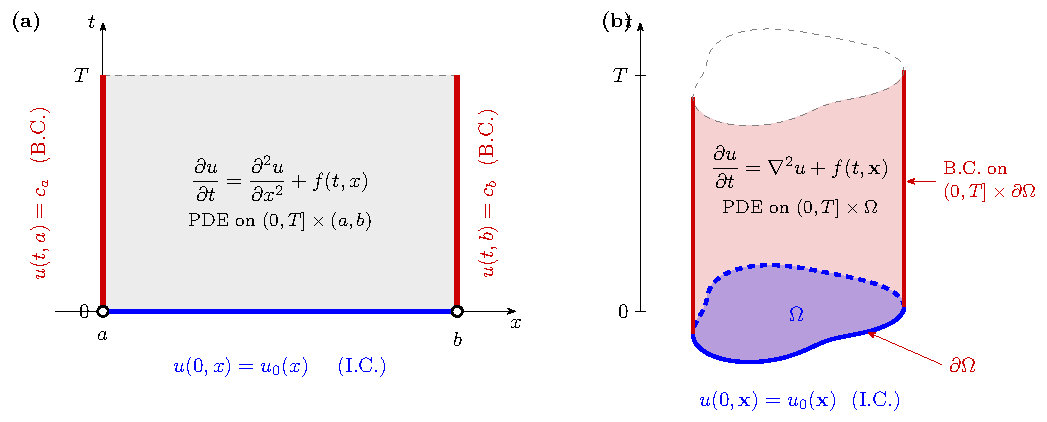
\includegraphics[width=\textwidth]{./Lectures/Lec21/heat_domain.pdf}
        \caption{Space-time domains of the heat equation. 
        (a) The one-dimensional problem \eqref{eq:heat-equation-1D}: the 
        PDE is imposed in the interior $(0,T] \times (a,b)$ (shaded), 
        the initial condition on the bottom edge $t = 0$ (blue), and 
        the boundary conditions on the lateral edges $x = a$ and 
        $x = b$ (red). The corners $(0,a)$ and $(0,b)$ (open circles) 
        are excluded from both. (b) The higher dimensional analogue: 
        the space-time cylinder $(0,T] \times \Omega$ over a domain 
        $\Omega \subseteq \R^d$ with smooth boundary $\partial\Omega$. 
        The PDE is imposed inside the cylinder, the initial condition 
        on its base $\{0\} \times \Omega$ (blue), and the boundary 
        conditions on its lateral surface $(0,T] \times \partial\Omega$ (red).}
        \label{fig:l21:heat-domain}
    \end{figure}

    \item (Elliptic PDEs) These are PDEs that 
    describe the steady-state or equilibrium 
    states of parabolic PDEs and hence do not have a 
    sense of time dependence or dynamics. Setting $\partial u/\partial t$ 
    in \eqref{eq:heat-equation} we obtain the Poisson PDE 
    which is perhaps to most well-known instance of an elliptic PDE: 
    \begin{equation}
        \begin{aligned}\label{eq:l21:poisson}
            - \nabla^2 u (\xb) & = f (\xb), && \xb \in \Omega \\
            u(\xb) & = c(\xb), && \xb \in \partial \Omega. 
        \end{aligned}
    \end{equation}
    Notice that no initial condition is needed now but we still need a 
    boundary condition. An example solution of the Poisson equation 
    is shown in the middle row of \Cref{fig:l21:pde-examples}.

    \item (Hyperbolic PDEs) These are PDEs that describe the 
    propagation of wave phenomenon or conservation laws. The 
    typical example is the wave equation 
    \begin{equation*}
        \begin{aligned}
        \frac{\partial^2 u}{\partial t^2}(t, \xb) &=
        \nabla^2 u(t, \xb)
        + f(t, \xb), && (t, \xb) \in (0, T] \times \Omega, \\
        u(0, \xb) & = u_0(\xb), \quad
        \frac{\partial u}{\partial t}(0, \xb) = v_0(\xb),
        && \xb \in \Omega \qquad \text{(I.C.)}, \\
        u(t, \xb) & = c(t, \xb), && t \in (0, T] \text{ and } \xb \in \partial \Omega
        \qquad \text{(B.C.)}.
        \end{aligned}
    \end{equation*}
    Since the PDE is second order in time we now need two initial
    conditions: the initial displacement $u_0$ and the initial
    velocity $v_0$. Snapshots of a numerical solution of the wave 
    equation are shown in the bottom row of \Cref{fig:l21:pde-examples}; 
    in contrast to the heat equation, the initial pulse does not 
    decay but propagates as a wave that reflects off the boundary.

    \begin{figure}[!htbp]
        \centering
        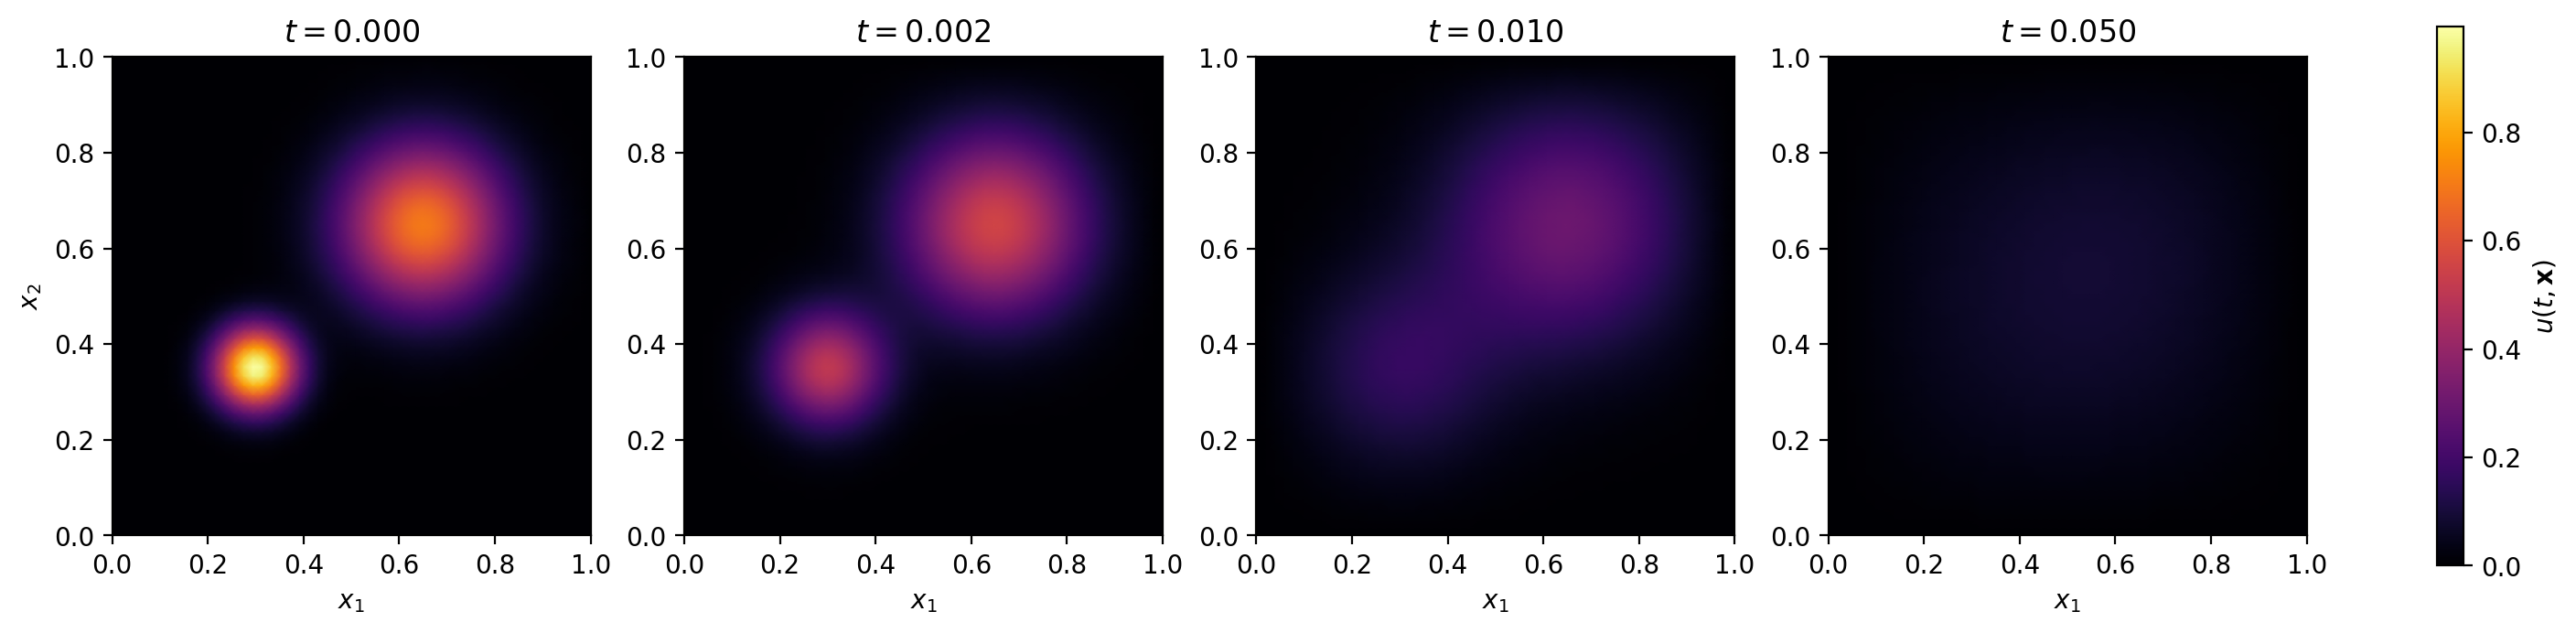
\includegraphics[width=\textwidth]{./Lectures/Lec21/heat_2d_snapshots.png}\\[0.5em]
        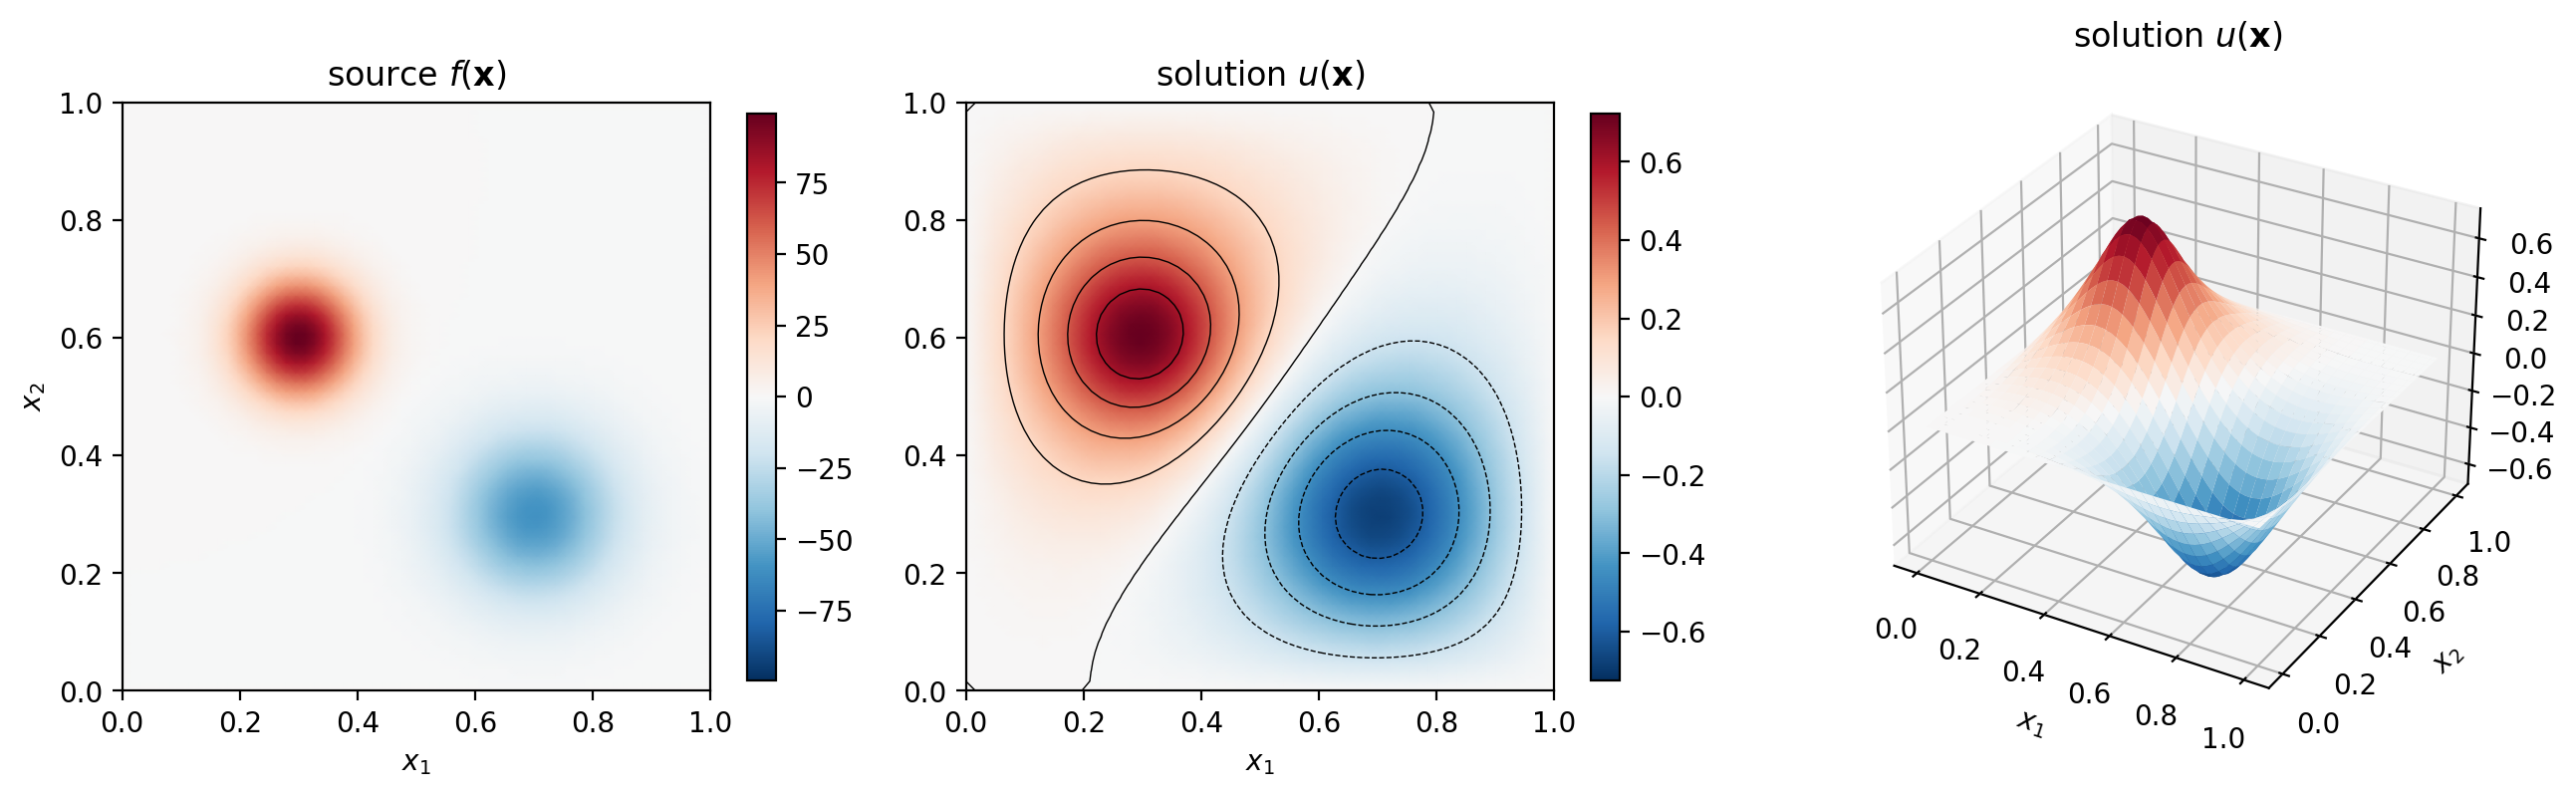
\includegraphics[width=0.9\textwidth]{./Lectures/Lec21/poisson_2d.png}\\[0.5em]
        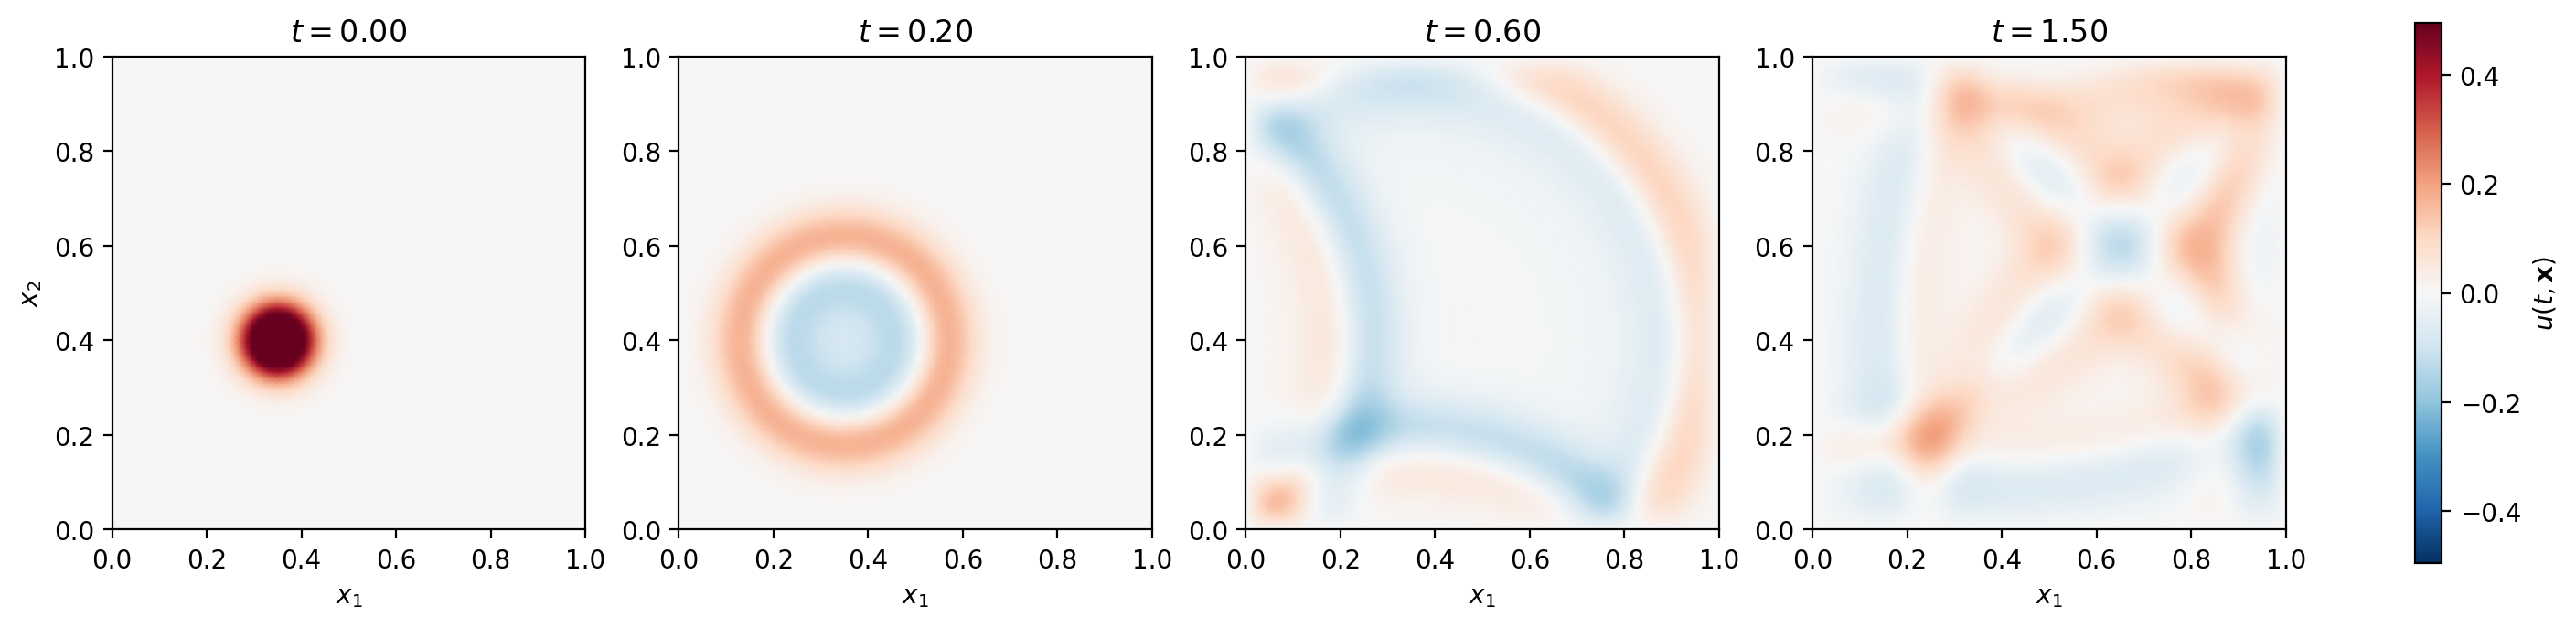
\includegraphics[width=\textwidth]{./Lectures/Lec21/wave_2d_snapshots.png}
        \caption{Numerical solutions of the three prototypical PDEs on 
        the unit square $\Omega = (0,1)^2$ with zero Dirichlet boundary 
        conditions. 
        (Top) The heat equation \eqref{eq:heat-equation} with $f = 0$ and 
        an initial condition made of two Gaussian bumps: the solution 
        diffuses, smooths out, and decays to zero. 
        (Middle) The Poisson equation $-\nabla^2 u = f$ with a source 
        $f$ consisting of a positive and a negative Gaussian bump (left) 
        and the resulting solution $u$ (center and right). 
        (Bottom) The wave equation with $f = 0$, an initial Gaussian 
        pulse $u_0$, and zero initial velocity $v_0 = 0$: the pulse 
        propagates outward as a ring and reflects off the boundary 
        without decaying.}
        \label{fig:l21:pde-examples}
    \end{figure}
\end{itemize}

Our goal in the rest of the course is to develop numerical algorithms for 
solving these three types of PDEs along with some of their nonlinear 
extensions. The key ideas that we will use will be very familiar given 
our previous encounter with IVPs and BVPs. For example, consider the 
heat equation \eqref{eq:heat-equation-1D} and discretize the problem 
in the $x$ variable only, using a uniform grid of size $\Delta x$ and
 centered differences, to get
\begin{equation*}
 \begin{aligned}
        \frac{\partial u}{\partial t}(t, x_i) 
   & = \frac{\partial^2 u}{\partial x^2}(t, x_i) + f(t, x_i) \\ 
   & \approx \frac{u(t, x_{i-1}) - 2 u(t, x_i) + u(t, x_{i+1})}{\Delta x^2}
   + f(t, x_i), 
 \end{aligned}
\end{equation*}
Now define $u_i(t) = u(t, x_i)$ and observe that the semi-discrete problem 
is simply describing a coupled system of ODEs 
\begin{equation*}
    u_i' = \frac{u_{i-1}(t) - 2 u_{i}(t) + u_{i+1}(t)}{\Delta x^2} + f_i(t),
\end{equation*}
along with an initial condition and hence is a IVP that we can solve 
using our earlier techniques. This is called the {\it method of lines}, i.e., 
a semi-discrete formulation of a dynamic PDE to turn it into an ODE system.
This ODE system turns out to be very stiff as we will see later on, and 
so many considerations from our discussion of ODEs remain relevant. 

Alternatively, we can approximate the whole PDE differential operator 
all at once, using finite differences, for example, consider 
\eqref{eq:l21:poisson} in 2D with $\Omega = (0,1) \times (0,1)$,
 write $\xb = (x, y)$ and consider a 2D uniform grid $(x_i, y_j)$ 
 for $x_i = i \Delta x$ and $y_j = j \Delta y$. Finally, write 
 $u_{i,j} = u(x_i, y_j)$. Then the Laplacian operator can be approximated as 
 \begin{equation*}
    \begin{aligned}
            \nabla^2 u(x_i, y_j) & = \frac{\partial^2 u}{\partial x^2}(x_i, y_j)
    + \frac{\partial^2 u}{\partial y^2}(x_i, y_j) \\
    & \approx \frac{u_{i-1, j} - 2 u_{i,j} + u_{i+1, j}}{\Delta x^2} 
    + \frac{u_{i, j-1} - 2 u_{i,j} + u_{i, j+1}}{\Delta y^2}.
    \end{aligned}
 \end{equation*}
This approximation is known as the {\it 5-point stencil} for the 
Laplacian since it couples each node $(x_i, y_j)$ only to its four 
nearest neighbors; see \Cref{fig:l21:laplacian-stencil}. 

\begin{figure}[!htbp]
    \centering
    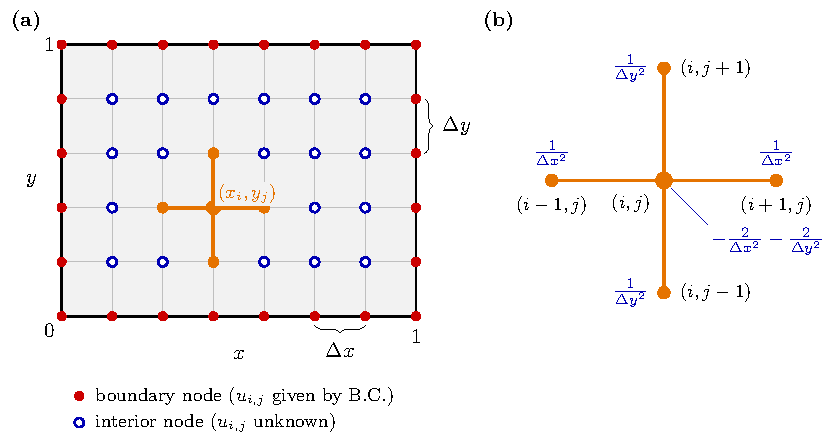
\includegraphics[width=\textwidth]{./Lectures/Lec21/laplacian_stencil.pdf}
    \caption{Finite difference discretization of the Laplacian on 
    $\Omega = (0,1)^2$. (a) A uniform grid with spacings $\Delta x$ and 
    $\Delta y$: the values $u_{i,j}$ at the boundary nodes (red) are 
    given by the boundary condition, while the values at the interior 
    nodes (blue) are unknown. The 5-point stencil centered at an interior 
    node $(x_i, y_j)$ is highlighted (orange). (b) The 5-point stencil 
    with the weights multiplying each $u_{i,j}$ in the approximation of 
    $\nabla^2 u(x_i, y_j)$.}
    \label{fig:l21:laplacian-stencil}
\end{figure}


% \bibliographystyle{plainnat}
% \bibliography{references}